\chapter{The FACET E210 Experiment}

\section{The FACET experimental setup}
\subsection{Laser energy calibration}
The FACET laser system ...
The energy that can be used on target of the OAP is controlled at two points in the laser-beamline.
At each point a cube-polarizer is surrounded by two  $\lambda/2$-waveplates, where the upstream one is motorized.
The main energy waveplate is located in the laser-room and the probe-energy waveplate is located in the tunnel area shortly after the split between main laser path and probe laser path at the main sampler, which means that the probe laser energy is determined by both waveplate settings while the main laser energy is set by the main laser energy waveplate only. From the power-meter in the laser-room, that measures shot-by-shot laser pulse energy, all the way down to the tunnel a variety of optical components are used until the laser is finally focused onto the 
The typical shot-to-shot laser energy jitter  is $\approx 5 \%$ FWHM.


\begin{figure}[htbp]
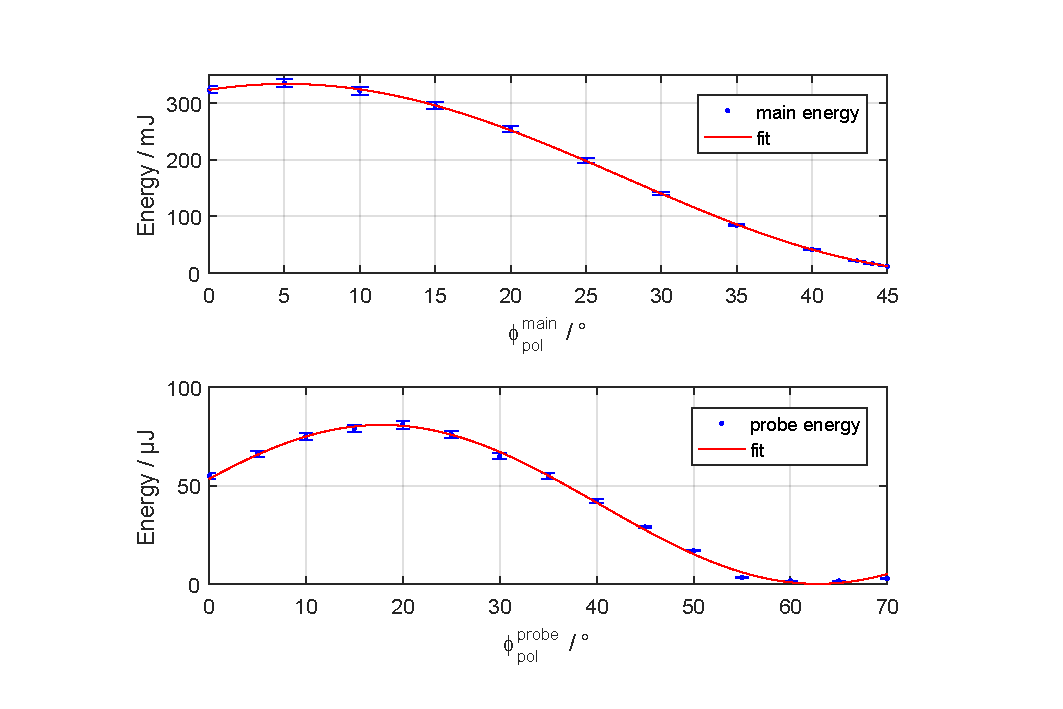
\includegraphics[width=0.9\textwidth]{experiment/images/edited/waveplate_calibration.pdf}
\caption{Laser energy calibration for main energy waveplate (upper plot) and probe energy waveplate (lower plot)}
\label{img:LaserEnergyCalib}
\end{figure}
All measured losses in optical components combined with the fitted functions for the waveplate energies (see figure \ref{img:LaserEnergyCalib}) combined give the on target energy applicable by axilens and OAP respecively.
\begin{align*}
 W_\mathrm{Laser}^\mathrm{OAP} &= W_\mathrm{Laser}^\mathrm{Laserroom}\times 1.25\times10^{-2}\\ &\times\big( 0.994 \cos^2(\frac{2\pi}{180} (\phi_{pol}^{main}+66.9)) +1.16\times 10^{-3}\big)\\
  &\times \big(0.998 \cos^2(\frac{2\pi}{180}(\phi_\mathrm{pol}^\mathrm{probe}-17.8 )) +1.62\times 10^{-3}\big)
\end{align*}

\begin{align}
 W_\mathrm{Laser}^\mathrm{Axilens} &= W_\mathrm{Laser}^\mathrm{Laserroom}\times 0.253\\ &\times\big( 0.994 \cos^2(\frac{2\pi}{180} (\phi_\mathrm{pol}^\mathrm{main}+66.9)) +1.16\times 10^{-3}\big)\\
\end{align}
This means that for a typical laser energy output of $500\, \mathrm{mJ}$ a maximum energy of $6.2\, \mathrm{mJ}$ on OAP target and $125.9\,\mathrm{mJ}$ on axilens could be used.


\section{Electro Optical Sampling (EOS)}

\section{Torch kick}
\begin{figure}[htbp]
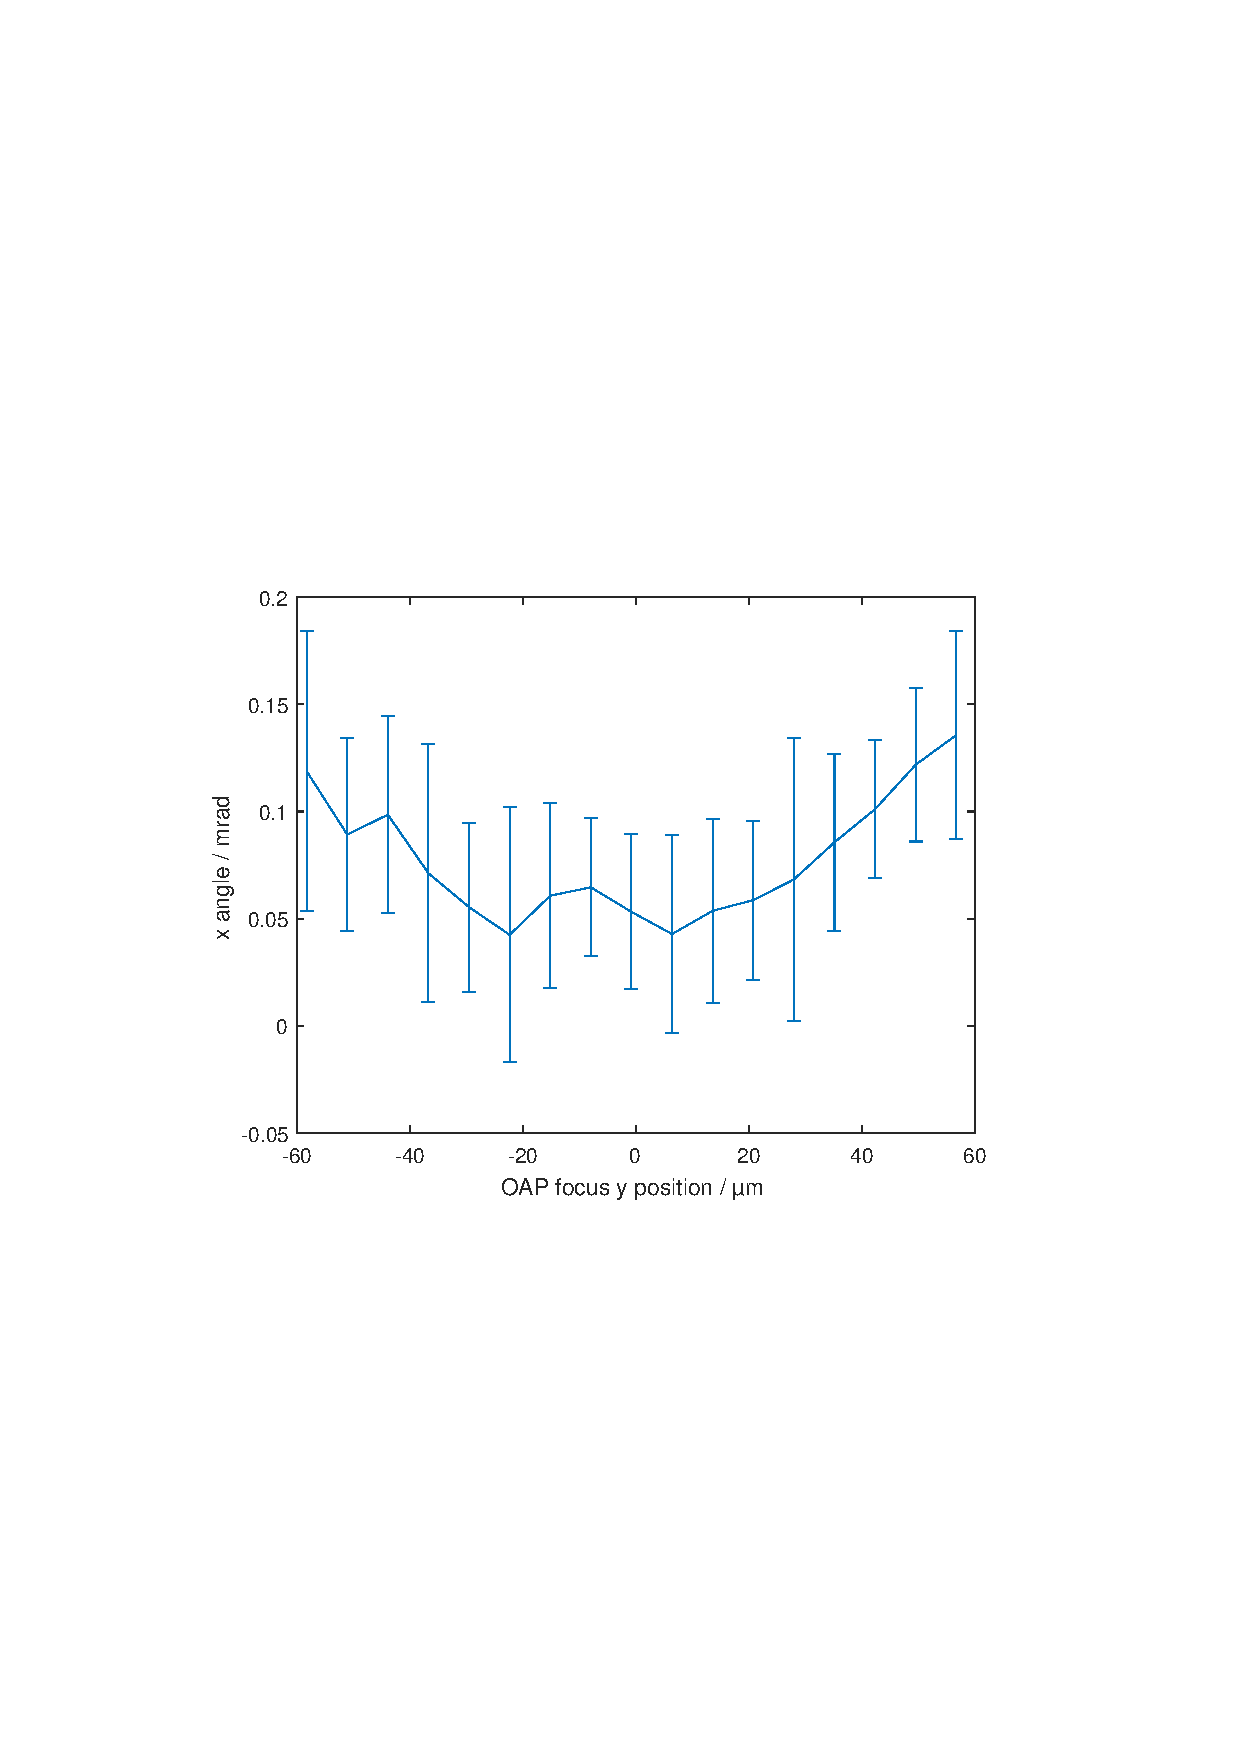
\includegraphics[width=0.9\textwidth]{experiment/images/raw/Torch_rollscan.pdf}
\caption{'test'}
\label{img:TochKick}
\end{figure}

\section{Ionization test}

\section{Plasma glow diagnostic}
One huge advantage of the hydrogen FACET setup compared to the oven setup is that now several view ports allow for observing the interaction or \ref{Facet_setup}.

The plasma glow diagnostic as a very simple tool, that turned out to be extremely helpful in controlling the 
alignment and synchronization of the experimental setup. The main idea is to have a camera integrate over the recombination light. It was observed that this 

%\section{FlashForwad}

\bibliography{lib}
